\section{Eksperymenty}
W tym rozdziale opisane zostaną eksperymenty przeprowadzone w celu zbadania testów wydajnościowych środowisk uruchomieniowych. Testy zostały przeprowadzone na jednym komputerze wyposażonym w system operacyjny Linux, co pozwoliło na zminimalizowanie wpływu innych czynników na wyniki testów. 

\subsection{Algorytmy sortowania}
W celu zbadania wydajności danego środowiska uruchomieniowego, skonstruowana odpowiednie eksperymenty, które sprawdzają wydajność algorytmu sortowania. Wszystkie algorytmu sortowania zostały przetestowane dla każdego środowiska. W tabeli \ref{tab:sorting_experiments} przedstawiono ilość iteracji oraz ilość eksperymentów dla przeprowadzonych eksperymenty.

\begin{table}[H]
  \centering
  \begin{tabular}{|c|c|}
    \hline
    \textbf{Liczba iteracji} & \textbf{Liczba elementów} \\ \hline
    10 & 1000 \\ \hline
    100 & 1000 \\ \hline
    1000 & 1000 \\ \hline
    10 & 10000 \\ \hline
    100 & 10000 \\ \hline
    1000 & 10000 \\ \hline
  \end{tabular}
  \caption{Parametry eksperymentów}
  \label{tab:sorting_experiments}
\end{table}

\subsubsection{Wyniki - sortowanie bąbelkowe}
\begin{figure}[H]
  \minipage{0.49\textwidth}
    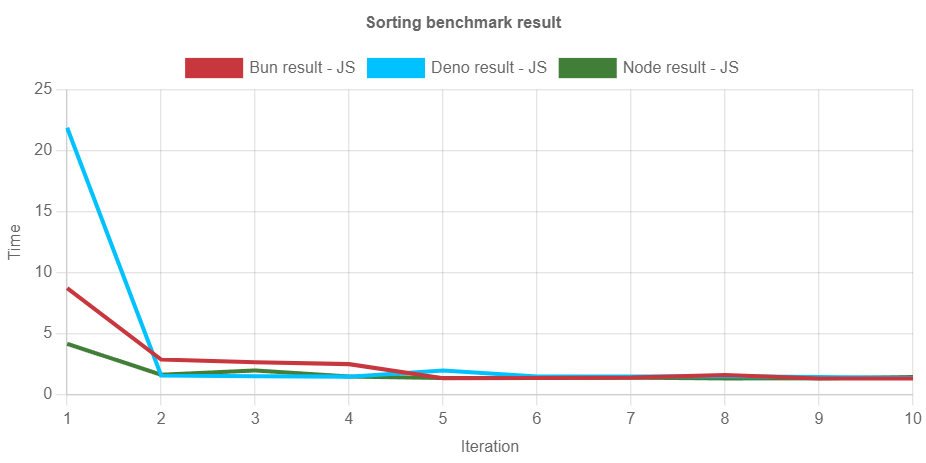
\includegraphics[width=\linewidth]{Figures/sorting/bubble/e1_js.png}
    \caption{Wyniki eksperymentów dla algorytmu sortowania bąbelkowego dla 10 iteracji i 1000 elementów}
    \label{fig:bubble_sorting_e1}
  \endminipage\hfill
  \minipage{0.49\textwidth}
  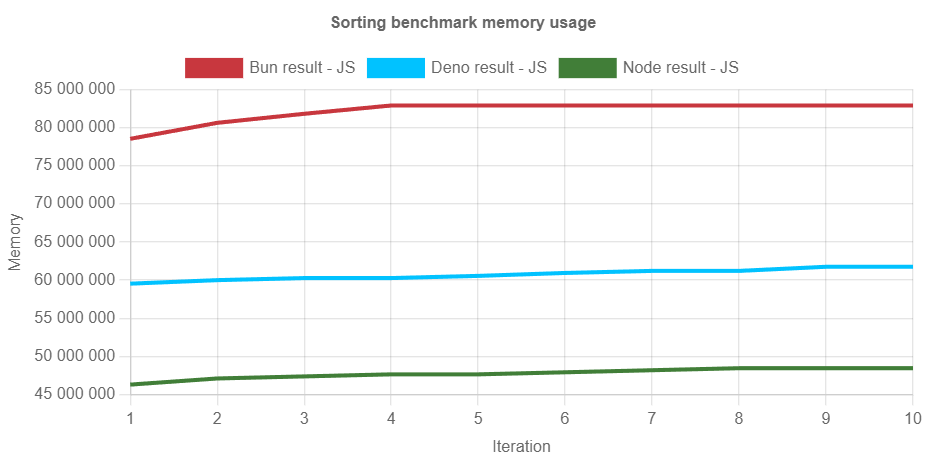
\includegraphics[width=\linewidth]{Figures/sorting/bubble/e1_memory_js.png}
  \caption{Wyniki eksperymentów dla algorytmu sortowania bąbelkowego dla 10 iteracji i 1000 elementów}
  \label{fig:bubble_sorting_e1_memory_js}
  \endminipage\hfill
\end{figure}

\subsection{Wyniki - sortowanie szybkie}

\subsubsection{Wyniki - sortowanie pozycyjne}

\subsection{Algorytmy kodowania}
W celu zbadania wydajności możliwości kodowania dla środowisk, użyto algorytmu kodowania Base64, który jest najpopularniejszym algorytmem kodowania wykorzystywanym w aplikacjach webowych. W tabeli \ref{tab:encoding_experiments} przedstawiono liczbę przeprowadzonych eksperymentów, długość kodowanego słowa.

\begin{table}[H]
  \centering
  \begin{tabular}{|c|c|}
    \hline
    \textbf{Liczba eksperymentów} & \textbf{Długość słowa}\\ \hline
    10 & 8192 \\ \hline
    100 & 32768 \\ \hline
  \end{tabular}
  \caption{Parametry eksperymentów}
  \label{tab:encoding_experiments}
\end{table}

\subsubsection{Wyniki}

\subsection{Testy wydajnościowe operacji zapisu i odczytu plików}

\subsubsection{Wyniki}

\subsection{Testy wydajnościowe serwera HTTP}

\subsubsection{Wyniki}

\subsection{Testy wydajnościowe zapisu i odczytu danych z bazy danych}

\subsubsection{Wyniki}